\documentclass[12pt]{article}
\usepackage{fullpage,enumerate,amsmath,amssymb,graphicx, float}

\begin{document}
\begin{center}
{\Large CS224N Fall 2014 Programming Assignment 2}
\vspace{12pt}

SUNet ID: tzhang54, jiajihu

Name: Tong Zhang, Jiaji Hu
\vspace{12pt}
\end{center}

\section{Implementing a CKY Parser}
\subsection{Algorithm and Naive Implementation}
To implement the CKY Parser, we followed the pseudocode introduced in the videos. The main idea of the algorithm is that we build up the parse in a bottom-up manner. During the process, we store intermediate results to speed up the process.
As introduced in the videos, the time complexity of the CKY algorithm is $O(n^3)$.

We started with a naive implementation of the algorithm. Note that the key design choices in the implementation is what kind of data structure we choose to store the intermediate results. In particular, the two tables \texttt{score} and \texttt{back}.

From the very start, it was clear that we cannot use a 3-d array to store these tables, as the third dimension will be very large but sparse, due to the large number of distinct words in the treebank, and we will quickly run out of memory. Therefore, we chose to use a Hashmap data structure. We chose \texttt{HashMap<Triplet<Integer, Integer, String>, Double>} for \texttt{score}, and \texttt{HashMap<Triplet<Integer, Integer, String>, Triplet<Integer, String, String>>} for \texttt{back}. Also, to keep track of which tags had non-zero values in a block, we kept a \texttt{HashMap<Pair<Integer, Integer>, Set<String>>} called \texttt{tagDict} to retrieve that set of tags.

Looking back, this setup was highly inefficient. Using the optimizations described below, we were able to dramatically improve our speed performance, resulting in a setup that could parse the test set in less than 3 minutes, averaging one parse per second, and handle sentences of length 20 in 2 seconds.
\subsection{Optimizations}
\subsubsection{Data Structures}
First, we came across the \texttt{CounterMap} data structure provided in the code library. We realized that it was quite convenient for our use case. Using a \texttt{CounterMap<Pair<Integer, Integer>, String>} for \texttt{score}, we were able to gt rid of \texttt{tagDict}, since the information was already in the Map.

Next, we looked into using \texttt{IdentityHashMap} to further improve the speed of operations in \texttt{score}. Since a data structure that incorporated \texttt{IdentityHashMap} into \texttt{CounterMap} was not provided, we wrote our own \texttt{IndentityCounterMap}, which used an \texttt{IdentityHashMap} in the first step, which is \texttt{Pair<Integer, Integer>} to \texttt{String}. We didn't use it for the \texttt{String} to \texttt{Double} step because we figured that we would then need an \texttt{Interner} for \texttt{String}, which might be computationally heavy and especially heavy on memory.

For the \texttt{back} table, we also wanted to incorporate \texttt{IdentityHashMap}. We had the idea that since we were already using an \texttt{Interner<Pair<Integer, Integer>>} for \texttt{score}, we might as well utilize that also for \texttt{back}. Therefore, we came up with a similar data structure to \texttt{IdentityCounterMap}, and named it \texttt{IdentityTripletMap}. Of course, we had to write that up ourselves.

Using these data structures, we were able to dramatically improve our runtimes. In addition, we were able to shave a bit more off our runtime by doing analysis on our code flow.
\subsubsection{Code Analysis}
We carefully analyzed our code to see if we could save a bit of computation here and there. For example, by moving our interning 

20\%
\subsection{Results}
\subsubsection{Run Time}
\begin{center}
\begin{tabular}{|c|c|c|c|}
\hline
Algorithm & Total Runtime (s) & Avg. Runtime (s) & Length 20 (s)\\\hline
Basic & 160.32 & 1.03 & 2.04 \\\hline

\end{tabular}
\end{center}
\begin{figure}[H]
\centering
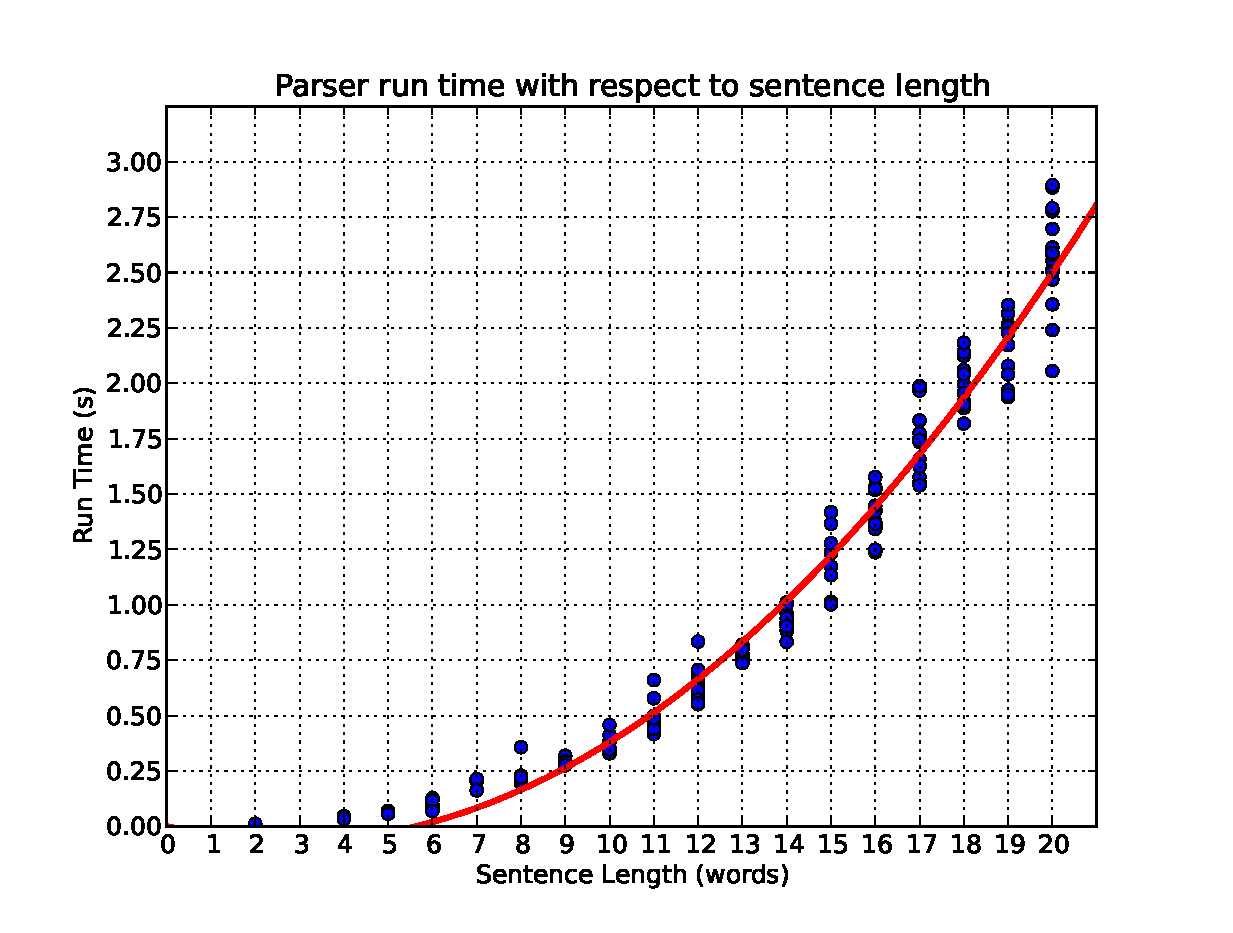
\includegraphics[width=0.6\linewidth]{./stats/runtime}
\end{figure}

\subsubsection{Parsing Score}
\begin{center}
\begin{tabular}{|c|c|c|c|c|}
\hline
Algorithm & Precision & Recall & $F_1$ & Exact Match \\\hline
Basic & 80.76 & 74.63 & 77.57 & 20.65\\\hline

\end{tabular}
\end{center}

\section{Adding Vertical Markovization}

\section{Extra Credit}

\end{document}